% This is a LaTeX tutorial by Overleaf titled [Learn LaTeX in 30 minutes](https://www.overleaf.com/learn/latex/Learn_LaTeX_in_30_minutes).

\documentclass[12pt, letterpaper, oneside]{report}
\usepackage[utf8]{inputenc}
\usepackage{graphicx}
\usepackage{amsmath}

\title{First document}
\author{Tran Phong Binh\thanks{phongbinh2511@gmail.com}}
\date{\today}

\begin{document}

\maketitle

\begin{abstract}
This is a simple paragraph at the beginning of the document. A brief introduction about the main subject.
\end{abstract}

\tableofcontents

\chapter{First Chapter}

\section{Introduction}
The first line after section is always fucked like this. Feels like an introduction to the section though.

First document. This is a simple example, with no extra parameters or packages included. Maybe if I put in more words, the difference between oneside and twoside will be revealed. I am not sure but this is what I would do. Unfortunately the experiment failed, I guess oneside and twoside implies a different meaning than what I have thought. Oh! I tried again, and it had nothing to do with the formatting of the content, but of the document itself! The margins are changed, they are shifted, together with the footnotes. I don't know if there are more things that change! So this is what working with \LaTeX{} feels like! Some of the \textbf{greatest} discoveries in \underline{science} were made by \textbf{\textit{accident}}. Below are some unordered lists stuff:
\begin{itemize}
    \item The individual entries are indicated with a black dot, a so-called bullet.
    \item The text in the entries may be of any length.
\end{itemize}
What if I want to continue the thing. Would I do it like this? Yes, yes it is. Now here it comes to the ordered lists:
\begin{enumerate}
    \item This is the first entry in our list
    \item The list numbers increase with each entry we add
\end{enumerate}
And then some texts follow that to be less awkward! In physics, the mass-energy equivalence is stated by the equation $E = mc^2$, discovered in 1905 by Albert Einstein. Again, the equation but in display mode will be written as
\[ E = mc^2 \]
for aesthetic. In natural units ($c = 1$), the formula expresses the identity
\begin{equation}
E = m
\end{equation}
Okay, that's cool. Now we are testing some texts after that.

\section{Second Section}
Well of-course this is the case too. Introduction stuff on the first line!

Some of the greatest \emph{discoveries}
in science were made by accident.

\begin{figure}[h]
    \centering
    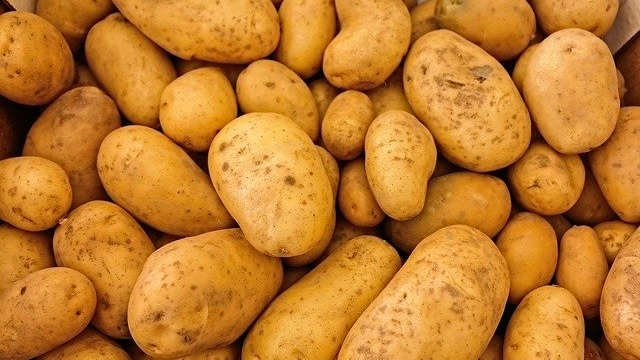
\includegraphics[width=0.25\textwidth]{potato}
    \caption{potato world}
    \label{bar}
\end{figure}

As you can see in the figure \ref{bar}, this is the world of potato. Also for your curiosity, page \pageref{bar} is the page of that image.

\subsection{First Subsection}
I mean like why not? Introduction on the first line seems cool.

\textit{Some of the greatest \emph{discoveries}
in science were made by accident.}

\textbf{Some of the greatest \emph{discoveries}
in science were made by accident.}

\section*{Unnumbered Section}
\addcontentsline{toc}{section}{Unnumbered Section Name On ToC}
Well maybe it will become uncool somehow, but for the matter of writting, this first line introduction seems like a good convention.

Subscripts in math mode are written as $a_b$ and superscripts are written as $a^b$. These can be combined an nested to write expressions such as
\[ T^{i_1 i_2 \dots i_p}_{j_1 j_2 \dots j_q} =
T( x^{x_1}, \dots, x^{i_p}, e_{j_1}, \dots, e_{j_q} ) \]

We write integrals using $\int$ and fractions using $\frac{a}{b}$. Limits are placed on integrals using superscripts and subscripts:
\[ \int_0^1 \frac{dx}{e^x} = \frac{e - 1}{e} \]

Lower case Greek letters are written as $\omega$ $\delta$ etc. while upper case Greek letters are written as $\Omega$ $\Delta$.

Mathematical operators are prefixed with a backslash as $\sin(\beta)$, $\cos(\alpha)$, $\log(x)$ etc.

\begin{center}
\begin{tabular}{ |c|c|c| }
    \hline
    cell1 & cell2 & cell3 \\
    cell4 & cell5 & cell6 \\
    cell7 & cell8 & cell9 \\
    \hline
\end{tabular}
\end{center}

Okay, I guess that's enough playing with toy table. It's time for some real shit. Table \ref{table:data} is an example of referenced \LaTeX{} elements.

\begin{table}[h!]
    \centering
    \begin{tabular}{ ||c|c c c|| }
        \hline
        No. & Col1 & Col2 & Col3 \\ [0.5ex]
        \hline \hline
        1 & 6 & 87837 & 787 \\
        2 & 7 & 78 & 5415 \\
        3 & 545 & 778 & 7507 \\
        4 & 545 & 18744 & 7560 \\
        5 & 88 & 788 & 6344 \\ [1ex]
        \hline
    \end{tabular}
    \caption{Table to test captions and labels}
    \label{table:data}
\end{table}

\end{document}
